\documentclass[a4paper,12pt]{article}
\usepackage[a4paper,margin=1in]{geometry}
\title{User Guide}
\author{SDP Group 15-H}
\usepackage{listings}
\usepackage{color}
\usepackage{graphicx}
\usepackage{parskip}
%\usepackage{titling}
\usepackage{array}
\usepackage{soul}
\usepackage{hyperref}
\usepackage{wrapfig}

\graphicspath{ {images/} }

\definecolor{dkgreen}{rgb}{0,0.6,0}
\definecolor{gray}{rgb}{0.5,0.5,0.5}
\definecolor{mauve}{rgb}{0.58,0,0.82}
\definecolor{lightgray}{rgb}{0.95,0.95,0.95}

\lstset{
  aboveskip=3mm,
  belowskip=3mm,
  showstringspaces=false,
  columns=flexible,
  basicstyle={\footnotesize\ttfamily},
  numbers=none,
  numberstyle=\tiny\color{gray},
  keywordstyle=\color{blue},
  commentstyle=\color{dkgreen},
  stringstyle=\color{mauve},
  breaklines=true,
  breakatwhitespace=true,
  tabsize=3,
  backgroundcolor=\color{lightgray},
}

\sethlcolor{lightgray}
\newcommand{\hg}[1]{\hl{\ttfamily #1}}

\begin{document}

\begin{titlepage}
    \begin{center}
        \vspace*{1cm}
        
        \Huge
        \textbf{User Guide}
        
        \vspace{0.5cm}
        \LARGE
        SDP Group 15-H
        
        \vspace{1.5cm}
        \normalsize
		Emilia Bogdanova\\
		Patrick Green\\
        Julijonas Kikutis\\ 
		David McArthur\\
		Aseem Narang\\
		Ankit Sonkar\\
        
        \vfill
        
        
        \vspace{0.8cm}
        
        \begin{figure}
    	\vspace*{-2.5em}
    	\centering
    	
\includegraphics[scale=.30]{logo.png}
		\end{figure}
        
        \Large
        The University of Edinburgh\\
        
    \end{center}
\end{titlepage}

\section{Installation}

\subsection{Cloning the repository and setting up} \label{setup}

To clone the repository, execute in terminal:
\begin{lstlisting}
$ git clone https://github.com/julijonas/venus.git
\end{lstlisting}

Then go to the root directory of the project and create a Python virtual environment which will contain a local copy of the libraries needed for this project:
\begin{lstlisting}
$ cd venus
$ virtualenv --system-site-packages env
$ source env/bin/activate
\end{lstlisting}

Install the \textit{pyserial} library which is used to send data to Arduino through RF stick:
\begin{lstlisting}
$ pip install pyserial
\end{lstlisting}

To set the persistent radio chip configuration for a new Arduino board, connect to the PC with an USB cable, execute \hg{screen /dev/tty0} in terminal, and enter the following commands substituting the appropriate group number and radio frequency band:

\begin{lstlisting}
+++
ATID0015
ATAC
ATRP1
ATAC
ATCN80
ATAC
ATWR
ARDN
\end{lstlisting}

To close \hg{screen}, press \textit{Ctrl+A} and then \textit{X}. The identical steps have to be performed for a new RF stick.

To program the Arduino to receive and execute messages, open the Arduino IDE by executing \hg{arduino} in terminal. You'll need to add three libraries which can be found under \texttt{arduino/} in the project directory: \textit{ArduinoSerialCommand}, \textit{SDPArduino}, \textit{SimpleTimer}. In order to add a library, go to
\hg{Sketch -> Import Library... -> Add Library...} and choose the library directory you want to import. Then open the Arduino file \texttt{arduino/arduino.ino} using \hg{File -> Open...} and upload it to the board using \hg{File -> Upload}.

\section{Hardware overview}

\subsection{Components}
\subsubsection{Motors}
The wheels are powered by NXT motors on a gear system of $2:1$. A reduction of power of one wheel can be caused by the gears slipping out of line. The driving motors are labelled 0 to 3 from the back right clockwise. Simple motions can be tested using the \texttt{move direction\_angle turn\_angle} command where direction\_angle defines the movement vector and turning\_angle defines the rotation whilst moving on that vector. the gears in the grabber can come out of line as well when crashing so insure that when open the enter arm span occurs. The grab has a motor on one arm and uses a gear ratio of $25:10:10:25$ to ensure each arm is opened at the same rate and in the correct direction. A mini motor is used for this and therefore the actual motion calibrated using a time step and not encoders. Please see the specification for an explanation of the kick. As it relies on timing the open grabber with a spin jammed grabber arms can reduce accuracy.

\subsubsection{Senors}

Each NXT motor is connected to the rotary encoder board see the specification for an image. The connections in the anticlockwise order from the top are: the I2C bus to the Arduino, back right motor, back left motor, front left motor, and front right motor. Using this board the information about the amount of rotations the motor has performed since the last query is available for the Arduino code as a separate integer for every motor. Every 5 ms the board is queried whether the target value has been reached. After the average of the rotary values of all four motors becomes greater or equal to the target value, the motors are stopped. If plugged in incorrectly motors will run continuously regardless of encoder value.

The light sensor is located above the grabber. The sensor returns a value associated with the reflected colors in its line of sight. Then the Arduino compares that value to a predefined threshold corresponding to the red ball. Sometimes a white line inside the pitch can be mistaken for the ball noticeable in the games as a random kick whilst in a state of grabbing. Ensure \texttt{query\_ball} is working before playing and adjust the threshold as outline in calibrations.

\subsection{Usage}

\subsubsection{Preparation for the match}

In order to turn the robot on, connect the battery pack to the power board. The pack consists of 10 AA rechargable batteries. Normally one fully charged battery pack would last for 7-10 minutes after which noticeable under-turning will occur. Ensure that the battery back is placed directly in the center as a change in weight distribution can cause the need for a recalibration of moving , turning and kicking.

To communicate with Venus the RF stick should be connected to the machine you are running the commands from. Then after performing steps described in "Running instructions" section, you will be able to operate the robot.

If you make any changes in the Arduino code, you need to upload them before running the commands (uploading instructions can be found in the "Installation" section above). Uploading can be done either via RF stick or the USB cable connected to the Arduino board. 

\section{Software overview}

\subsection{Running instructions}

Run the following command in the terminal from the project root directory if it has not been done already to enable the Python virtual environment which contains the required libraries:
\begin{lstlisting}
$ source env/bin/activate
\end{lstlisting}

In order to set the room containing the pitch, colors of the robot, and side of the goal, change the hard-coded parameters of \textit{init} method in \textit{control/holonomic.py} as detailed in Table \ref{tab:params}.
For example, if the room is 3.D04, the robot has the yellow team color and one green-coloured dot, and the robot is defending the goal closer to the computers, the line would be:
\begin{lstlisting}
def init(self, room_num=1, team_color='yellow', our_color='green', computer_goal=True):
\end{lstlisting}

\begin{table}[h!]
\centering
\begin{tabular}{ | l | l | l | l | l | l | l | l | }
    \cline{1-2} \cline{4-4} \cline{6-6} \cline{8-8}
    Room & \texttt{room\_num} & & \texttt{team\_color} & & \texttt{our\_color} & & \texttt{computer\_goal} \\ 
    \cline{1-2} \cline{4-4} \cline{6-6} \cline{8-8}
    3.D03 & 0 & & 'yellow' & & 'green' & & True \\ 
    \cline{1-2} \cline{4-4} \cline{6-6} \cline{8-8}
    3.D04 & 1 & & 'blue' & & 'pink' & & False \\ 
    \cline{1-2} \cline{4-4} \cline{6-6} \cline{8-8}
\end{tabular}
\caption{Allowed parameters for the \textit{init} method}
\label{tab:params}
\end{table}

Then ensure that the RF stick is plugged in. To start the application, make connections to the RF stick, vision feed, and get access to the command prompt, execute the following line:
\begin{lstlisting}
$ python main.py
\end{lstlisting}

\textbf{NB}: In case you make changes to the Arduino code, you should upload your changes to the board as detailed in Section \ref{setup}.

Then the operator of the robot can start entering the commands. The main command is \hg{hs} which starts the strategy. The listing of all commands is provided in Table \ref{tab:commands}.

\begin{table}[h!]
\centering
\begin{tabular}{ | p{9cm} | p{6.2cm} | }
    \hline
    Constantly run the strategy state machine &
    \small{\texttt{hs}} \\ \hline
%    Set configuration values &
%    \small{\texttt{init room\_num team\_color our\_color computer\_goal}} \\ \hline
%    Connect to the RF stick &
%    \small{\texttt{connect}} \\ \hline
%    Start the vision &
%    \small{\texttt{vision}} \\ \hline
    Output a picture of the potential field of the state &
    \small{\texttt{map state\_name}} \\ \hline
    Perform a holonomic motion (angles in degrees) &
    \small{\texttt{move direction\_angle turn\_angle}} \\ \hline
    Move forward (in cm, negative means backward) &
    \small{\texttt{f distance}} \\ \hline
    Rotate clockwise (in degrees, negative means anticlockwise) &
    \small{\texttt{c angle}} \\ \hline
    Stop all motors &
    \small{\texttt{s}} \\ \hline
    Open the grabber &
    \small{\texttt{o}} \\ \hline
    Close the grabber &
    \small{\texttt{g}} \\ \hline
    Perform a spin kick &
    \small{\texttt{ee}} \\ \hline
    Print world state &
    \small{\texttt{w}} \\ \hline
    Query light sensor &
    \small{\texttt{query\_ball}} \\ \hline
    Pass the ball to the teammate &
    \small{\texttt{pass\_ball}} \\ \hline
    Catch the ball coming from the teammate &
    \small{\texttt{catch\_ball}} \\ \hline
    Kick the ball to the goal &
    \small{\texttt{goal}} \\ \hline
    Exit the application &
    \small{\texttt{exit}} \\ \hline
\end{tabular}
\caption{Commands available for the operator of the robot}
\label{tab:commands}
\end{table}

\texttt{goal} and \texttt{pass\_ ball} are the robots shooting command. First the optimum orientation of the robot is met. Then a second grab is initiated and the finally kick initiated through the \texttt{ee} command. Sleep is added before the kick to reduce irregularities in motor powers from previous movement. The \texttt{catch\_ball} command moves the robot to face its team mate. A grab is initiated once vision detects that the ball is within a range of 32cm set exactly for that camera speed. If the ball never enters this range and stops moving, vision will also detect this breaking out of the while loop instantly. The \texttt{ee} command instigates a kick by opening the grabber and spinning for an encoder value of 200, in that order. Irregularities in accuracy can come from both running over tape and also battery power.


\subsection{Calibration of the vision} \label{calibration}

\begin{wrapfigure}{r}{0.25\textwidth}
\centering
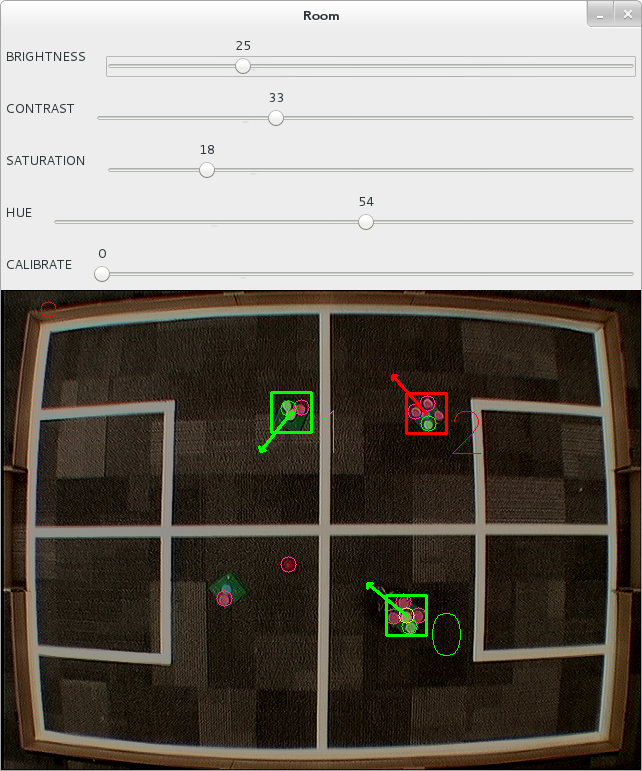
\includegraphics[scale=0.25]{images/calibration1.png}
\end{wrapfigure} 
\textbf{Camera capture settings}: As the images appearance can change between computers you may need to slightly adjust the capture settings. This simple calibration is always more preferable than going for a complete calibration. In which case use the slider bars that pop up on the vision feed each corresponding to a percentage see the image to the left. Brightness and contrast can help make the colors more distinguishable and a larger contrast than brightness works better. Reducing the saturation can help remove unwanted spots from the blurred colors created by the white lines.   
 
\textbf{Color calibration}: To enter this mode the slider bar named calibration must be moved. The first step is to click and the terminal will outline everything that can be calibrated, see image bellow. Each one is activated by pressing a key outlined bellow. For colors it is advised to click on that coloured spot a few times. Be sure to check the terminal to make sure your on the right color. For pitch dimensions a description of how to click each object is added in the terminal. The general convention is any order to mark the goals and for shapes start at the top left and work clockwise. Once you ready to move on press the ESC key. 

\begin{minipage}{0.5\textwidth}
\centering
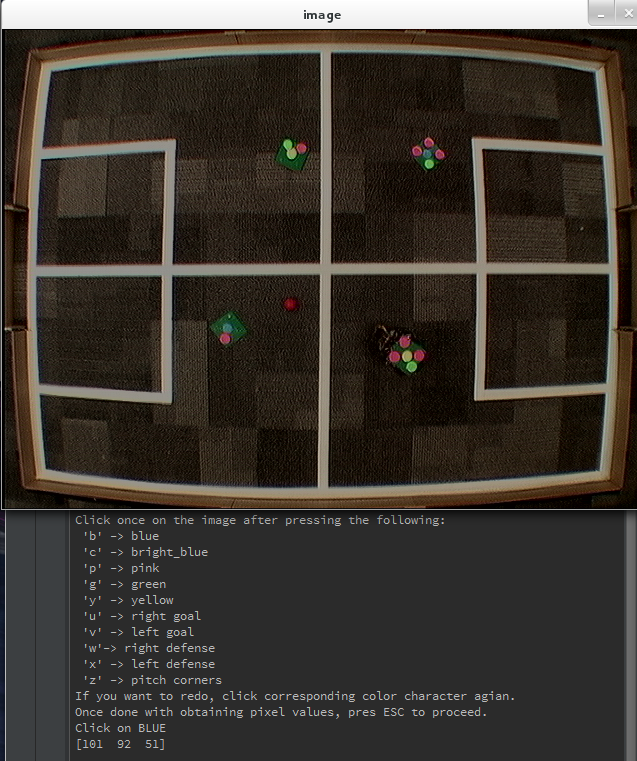
\includegraphics[scale=0.25]{images/calibration2.png}
\end{minipage}
~
\begin{minipage}{0.5\textwidth}
\centering
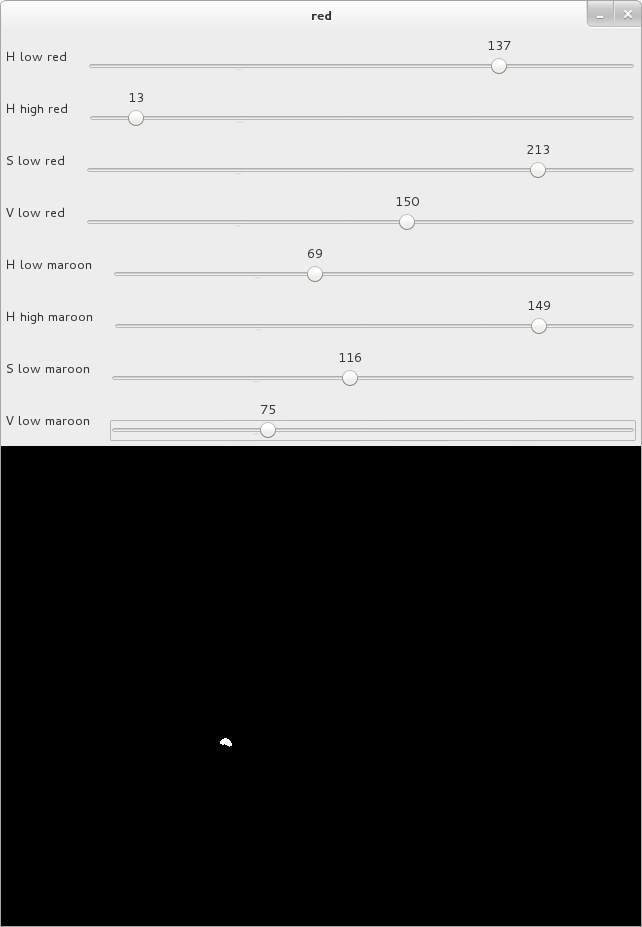
\includegraphics[height=200px]{images/calibration3.png}
\end{minipage}

\textbf{Fine tuning the colors}: Once the ESC key has been pressed the color thresholds predicted from the clicking can be fine tuned in the window shown above. If nothing is visible, it is advised to reduce saturation and value first before adjusting the hue values. The aim is to see as minimal of spots not in that color as possible and make the actual color as solid as possible. Press the ESC key to move on and eventually the original vision key will be brought up.

\textbf{Green and yellow}: As they can blend together easily it is important that they can be seen clearly so try to reduce the hue threshold of yellow and increase the hue threshold of green as much as possible. 

\textbf{Red and pink}: Sometimes the ball cannot be found so if you enter the calibration and press ESC instantly you will only be adjusting reds thresholds. The tuning window for red requires you to adjust to separate ranges of values so make sure this is done to get as clear spot as possible.  Its similarities with pink can be avoided after calibrating by adjusting the slider bars for the camera capture settings.      

\subsection{Handling} \label{handling}

Handle the robot with care. It is advisable not to lose the top plate during the game. It can be secured properly to the robot using Blu-Tack. 

\subsubsection{Calibration}

Before playing a match, ensure that the spin-kick (\texttt{goal} command), going forward (\texttt{f} command), and turning (\texttt{c} command) are calibrated. It can be done by repeatedly executing the respective commands with different input values, changing the data points in the \texttt{calibration.ods} spreadsheet, and changing the equations in \texttt{ee}, \texttt{f}, and \texttt{c} methods in \texttt{control/holonomic.py} to respective new computed equations from the spreadsheet. 

\begin{wrapfigure}{r}{0.3\textwidth}
\centering
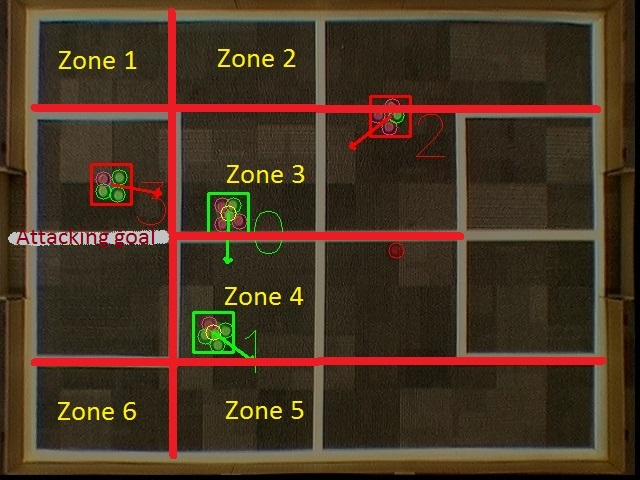
\includegraphics[scale=.4]{zones.jpg}
\caption{Different shooting zones}
\label{fig:zones}
\end{wrapfigure}

When calibrating the spin-kick the aim is for the robot to be not fully turned towards the goal before the kick. To achieve that, there are different "correction angles" for six main zones of the pitch (Figure  \ref{fig:zones}). These angles can be calibrated in \texttt{strategy/simple\_holonomic.py} in \texttt{shot\_correction} method. 

The best strategy here would be to place robot with the ball in different sections of one zone and execute the \texttt{goal} command choosing the constant for the angle that achieved the best result.

Another important action is checking whether the light sensor threshold correctly identifies the grabbed ball and lack thereof. The threshold is defined in \texttt{query\_ball} method in \texttt{control/holonomic.py}.

\textbf{NB}: If another robot is doing the kick-off in a game, do not start the strategy by typing \hg{hs} before that robot performs the kick-off.

\section{Troubleshooting guide}

\textbf{Problem 1}: When uploading the code to the Arduino board, the following error message appears:
\begin{lstlisting}
processing.app.SerialNotFoundException: Serial port '<port>' not found. Did you select the right one from the Tools > Serial Port menu?
\end{lstlisting}
\textbf{Solution}: Make sure you are not running the Python application at the same time or have not opened the serial interface any other way when the changes are being uploaded. The Arduino IDE is only able to program the Arduino when the serial interface of the RF stick or Arduino itself is registered as \texttt{/dev/ttyACM0} on the PC. If there are other programs accessing \texttt{/dev/ttyACM0} and the RF stick or USB cable is unplugged and plugged again, the "new" device is issued \texttt{/dev/ttyACM1} instead by the Linux kernel.

\textbf{Problem 2}: When sending commands the robot does not respond to any commands although it should move.

\textbf{Solution}: Power cycle the Arduino board.

\textbf{Problem 3}: The Python application cannot connect to the RF stick because the RF stick has registered itself as \texttt{/dev/ttyACM1}.

\textbf{Solution}: Either close all programs that have handles to \texttt{/dev/ttyACM0} and reconnect the RF stick or change the \texttt{device\_no} parameter in the \texttt{connect} method in \texttt{control/holonomic.py} to 1 and restart the Python application.

\textbf{Problem 4}: The commands are evidently sent but the robot does not move.

\textbf{Solution}: Power cycle the Arduino. If that does not help, change the battery set to a fully charged one.

\end{document}